
\begin{center}
\Huge
Mængder
\end{center}

\section*{Mængder}
\stepcounter{section}
Vi vil i forbindelse med funktionsbegrebet gerne introducere det meget brugbare begreb \textit{mængder}. Disse kan bestå af alle mulige objekter, men vil oftest bestå af tal, når vi taler om dem. Andre typer af objekter kunne være udfaldet \textit{plat}, hvis der kastes med en mønt.  

Vi starter med en definition, der er præcis nok til vores forståelse.
\begin{defn}[Mængde]
En mængde er en samling af \textit{entydige} elementer. 
\end{defn}
Bemærk, at ordet \textit{entydige} betegner, at et element kun kan optræde én gang i en mængde. 
\begin{exa}
	Følgende er eksempler på endelige mængder:
	\begin{align*}
		A &= \{a,b,c\},\\
		B &= \{2,3,banan,æble\},\\
		C &= \{1,2,3,\hdots,9,10\}.
	\end{align*}
	$A,$ $B$ og $C$ er navnene på mængderne, og tuborg-klammerne $\{\}$ bruges til at notere, at vi har med en mængde at gøre. Elementerne i mængden $A$ vil være $a$, $b$ og
	$c$. Udeladelsesprikkerne $\cdots$ bruges til at notere, at der er flere elementer i mængden end opskrevet og at læseren dermed selv skal udfylde hullet. 
\end{exa}
Mængder behøver som i eksemplet ikke at være endelige. De eksempler, I har set på mængder i 1.g er uendelige.

\begin{exa}
Vi vil arbejde med følgende vigtige mængder:
\begin{enumerate}[label=\roman*)]
\item Der er en mængde, der ingen elementer har. Denne mængde kaldes den tomme mængde og noteres med $\emptyset$ eller $\{\}$. 
\item Mængden af naturlige tal $\mathbb{N} = \{0,1,2,3,\hdots\}$.
\item Mængden af hele tal $\mathbb{Z} = \{\hdots,-3,-2,-1,0,1,2,3,\hdots \}$.
\item Mængden af alle rationale tal/heltalsbrøker $\mathbb{Q} = \left\{\frac{a}{b} \ \middle | \ a,b\in \mathbb{Z}, b \neq 0\right\}$. Eksempler er $1/2, 4, 27/3$
\item Mængden af reelle tal $\mathbb{R}$, der består af alle rationale tal og alle uendelige decimalfølger. Eksempler er $\textnormal{e},\pi, \sqrt{2}$
\end{enumerate}
\end{exa} Bemærk, at de rationale tal er skrevet op på formen $\mathbb{Q} = \left\{ \frac{a}{b} \ \middle | \ a,b \in \mathbb{Z}, b \neq 0 \right\}$. Denne notation kaldes typisk for \textit{mængdebyggernotation}, og skal forstås som 
\begin{align*}
	A = \{ \textnormal{Elementer} \mid  \textnormal{Betingelse}\}.
\end{align*}
Hvis en mængde $A$ er indeholdt i en mængde $B$, så skriver vi $A\subseteq B$ og $A$ kaldes en delmængde af $B$. To mængder er ens, hvis de indeholder hinanden, altså $A\subseteq B$ og $B\subseteq A$ og vi skriver $A=B$. 
\begin{exa}
Vi har følgende eksempler på delmængder:
\begin{enumerate}[label=\roman*)]
\item Mængden af alle mennesker er en delmængde af alle pattedyr som igen er en delmængde af alle dyr.
\item $\{1,2,3\} \subseteq \{1,2,3,4\}$.
\item De lige tal er en delmængde af de hele tal.  
\item $\{10,20\}\subseteq \{10,20\}$.
\end{enumerate}
\end{exa}
\begin{exa}[Den tomme mængde]
	Mængden, der ikke indeholder nogle elementer kaldes for \textit{den tomme mængde} og betegnes med $\{\}$ eller $\emptyset$. Det gælder for enhver mængde $A$, at 
	$\emptyset \subseteq A$.
\end{exa}

\section*{Mængdeoperationer}
Har vi to mængder, kan vi gøre os overvejelser om, hvordan disse mængder kan sammenlignes, og hvordan vi kan danne nye mængder ud fra gamle. 

\begin{defn}[Fællesmængde]
	Fællesmængden mellem to mængder $A$ og $B$ er den mængde, der består af de elementer, som begge mængder har til fælles. Mængden betegnes med $A \cap B$, og defineres mere
	præcist som
	\begin{align*}
		A \cap B = \{x \mid x \in A \land x \in B\}
	\end{align*}
\end{defn}

\begin{exa}\label{exa:1}
	Eksempler på fællesmængder er:
	\begin{enumerate}[label=\roman*)]
		\item $\{1,2,3\} \cap \{2,3,4\} = \{2,3\}$.
		\item $\{1,2,3\} \cap \{4,5,6\} = \emptyset$.
	\item      $\{$Pattedyr$\}$ $\cap$ $\{$Havdyr$\}$ = $\{$Hvaler, Sæler, Søkøer, Isbjørne, Havoddere$\}$
	\end{enumerate}
\end{exa}

\begin{defn}[Foreningsmængde]
Foreningsmængden af to mængder $A$ og $B$ består af de elementer, der er i enten $A$ eller $B$ og betegnes $A \cup B$. Mængden defineres mere præcist som
\begin{align*}
	A \cup B = \{x \mid x \in A \lor x \in B\}.
\end{align*}
\end{defn}
\begin{exa}
Vi har følgende eksempler på foreningsmængder:
\begin{enumerate}[label=\roman*)]
\item $\{1,2,3\} \cup \{4,5,6\} = \{1,2,3,4,5,6\}$.
\item $\{1,2\} \cup \{1,2,3,4\} = \{1,2,3,4\}$.
\item $\{$Ulige tal $\}$ $\cup$ $\{$Lige tal$\}=\mathbb{Z}$ 
\end{enumerate}
\end{exa}
\begin{defn}
Mængdedifferencen af to mængder $A$ og $B$ betegnes
\begin{align*}
A \backslash B
\end{align*}
og betegner de elementer, der er i $A$, men ikke i $B$. Bemærk at $A\backslash B$ og $B \backslash A$ generelt er forskellige.
\end{defn}

Vi har ofte brug for en mængde, der indeholder alle interessante elementer i en eller anden sammenhæng. Denne kaldes for universalmængden og betegnes med $U$. 
\begin{defn}
Komplementærmængden til en mængde $A$ betegnes med 
\begin{align*}
A^C 
\end{align*}
og defineres som $U\backslash A$. 
\end{defn}
\begin{exa}
Hvis $U$ består af mængden af udfald af et terningeslag $U=\{1,2,3,4,5,6\}$ og $A$ er mængden af udfald $A=\{1,2\}$, så vil komplementærmængden $A^C$ af $A$ være det, der er i $U$, men ikke i $A$, altså $A^C = U\backslash A = \{3,4,5,6\}$.
\end{exa}
Et brugbart redskab til at visualisere mængder og mængdeoperationer er Venn-diagrammer. Inklusionsforholdet mellem $\mathbb{N}, \mathbb{Z}, \mathbb{Q}$ og $\mathbb{R}$ kan ses af Venn-diagrammet på Fig. \ref{fig:venn1}
\begin{figure}[H]
\centering
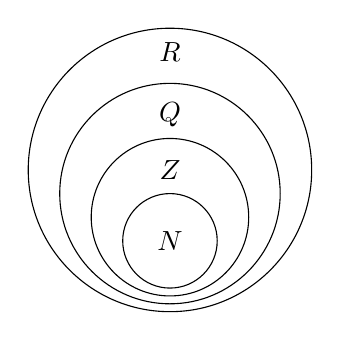
\begin{tikzpicture}
\draw (0.0,0.0) circle (0.6);
\draw (0.0,0.3) circle (1);
\draw (0.0,0.6) circle (1.4);
\draw (0.0,0.9) circle (1.8);
\node at (0,0) {$\mathbb{N}$};
\node at (0,0.9) {$\mathbb{Z}$};
\node at (0,1.6) {$\mathbb{Q}$};
\node at (0,2.4) {$\mathbb{R}$};
\end{tikzpicture}
\caption{Inklusionsforhold mellem $\mathbb{N},\mathbb{Z},\mathbb{Q}$ og $\mathbb{R}$.}
\label{fig:venn1}
\end{figure}
Fig. \ref{fig:Maengdeop} beskriver mængdeoperationer med Venn-diagrammer. 
\begin{figure}[H]


 \centering
 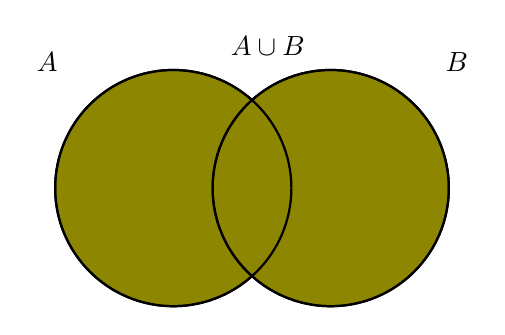
\begin{tikzpicture}[thick,
    set/.style = { circle, minimum size = 3cm}]

\draw[fill=olive] (0,0) circle (1.5cm);
\draw[fill = olive] (2,0) circle (1.5cm);
\draw[] (0,0) circle (1.5cm);
\draw (2,0) circle (1.5cm);

\node at (1.2,1.8) {$A\cup B$};
\node at (-1.6,1.6) {$A$};
\node at (2+1.6,1.6) {$B$};
\end{tikzpicture}
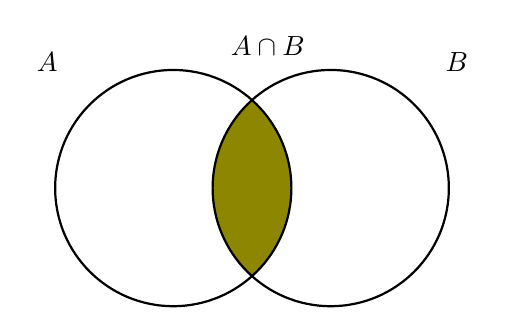
\begin{tikzpicture}[thick,
    set/.style = { circle, minimum size = 3cm}]


\node at (1.2,1.8) {$A\cap B$};
\node at (-1.6,1.6) {$A$};
\node at (2+1.6,1.6) {$B$};

\begin{scope}
    \clip (0,0) circle(1.5cm);
    \clip (2,0) circle(1.5cm);
    \fill[olive](0,0) circle(1.5cm);
\end{scope}
\draw[] (0,0) circle (1.5cm);
\draw[] (2,0) circle (1.5cm);
\end{tikzpicture}

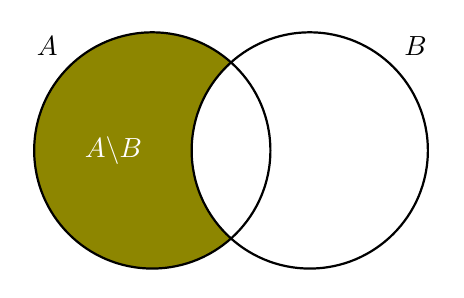
\begin{tikzpicture}[thick,
    set/.style = { circle, minimum size = 3cm}]
 
% Set A
\node[set,fill=olive,label={135:$A$}] (A) at (0,0) {};
 
% Set B
\node[set,fill=white,label={45:$B$}] (B) at (0:2) {};
 
% Circles outline
\draw (0,0) circle(1.5cm);
\draw (2,0) circle(1.5cm);
 
% Difference text label
\node[left,white] at (A.center){$A \backslash B$};
 
\end{tikzpicture}
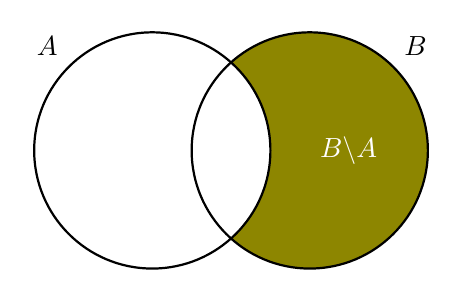
\begin{tikzpicture}[thick,
    set/.style = { circle, minimum size = 3cm}]
 
% Set B
\node[set,fill=olive,label={45:$B$}] (B) at (0:2) {};
 
% Set A
\node[set,fill=white,label={135:$A$}] (A) at (0,0) {};
 
% Circles outline
\draw (0,0) circle(1.5cm);
\draw (2,0) circle(1.5cm);
 
% Difference text label
\node[right,white] at (B.center){$B\backslash A$}; 
\end{tikzpicture}
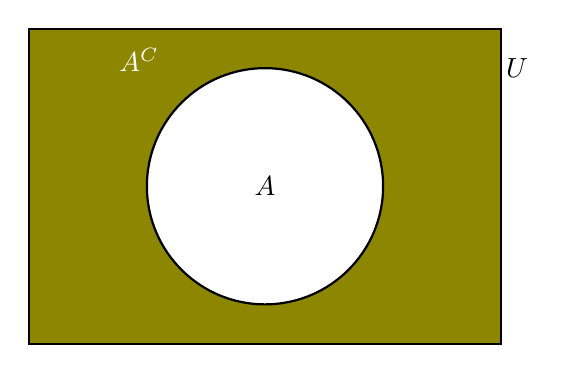
\begin{tikzpicture}[thick,
    set/.style = { circle, minimum size = 3cm}]
\draw[fill = olive] (-3,0) rectangle (3,4);
\draw[fill = white] (0,2) circle (1.5cm);

\node[] at (3.2,3.5) {$U$};
\node at (0,2) {$A$};
\node[white] at (-1.6,1.6+2) {$A^C$};
\end{tikzpicture}
\caption{Mængdeoperationer beskrevet med Venn-diagrammer}
\label{fig:Maengdeop}
\end{figure}

Til slut skal vi også introducere mængdetypen \textit{produktmængde}, der er vigtig, når vi skal tale om udfaldsrum for uafhængige i forbindelse med sandsynlighedsregning.
\begin{defn}[Produktmængde]
For to mængder $A$ og $B$ består produktmængden $A \times B$ af alle par
\begin{align*}
	\{(a,b) \mid a\in A, b \in B\}.
\end{align*}
Hvis $A = B$, skrives produktmængden også $A^2$.
\end{defn}
\begin{exa}
	Lad $A = \{1,2\}$ og $B = \{a,b\}$. Så består mængden $A \times B$ af elementerne
	\begin{align*}
		A \times B = \{(1,a),(1,b),(2,a),(2,b)\}.
	\end{align*}
\end{exa}
\begin{exa}
	Hvis mængden $A = \{K,P\}$ består af udfaldene af et møntkast, så vil mængden $A^2$ være
	\begin{align*}
		A^2 = \{(K,P),(P,K),(K,K),(P,P)\}.
	\end{align*}
\end{exa}
\begin{exa}
	Mængden $\mathbb{R}^2$ består af alle punkter i et sædvanligt koordinatsystem med to koordinatakser. 
\end{exa}

\subsection*{Opgave 1}
Bestem følgende mængder:
\begin{align*}
&1) \ \{7,9\} \cup \{9,4\}  &&2) \ \{1,3\} \backslash \{1,3\}    \\
&3) \ \{\textnormal{Banan},\textnormal{Æble}\} \backslash \{\textnormal{Pære},\textnormal{Banan},\textnormal{Agurk}\} &&4) \ \{1,2,3\} \cap \{3,4,5\}  \\
&5) \ \{a,b,c\} \cup \{c,d,e\}  &&6) \ \{a,b,c\} \cap \{c,d,e\}   \\
&7) \ (\{1,5,4,7 \} \cup \{5,6,1\}) \backslash \{1,2,3,4\}  &&8) \{2,3,5,7,11\} \cup \{2,4,6,8,10\}
\end{align*}
\subsection*{Opgave 2}
Tegn Venn-diagrammer, hvor det er opfyldt, at 
\begin{enumerate}[label = \roman*)]
	\item $A \cap B = A$,
	\item $A \cup B = A$,
	\item $A \backslash B = A$,
	\item $A \backslash B = \emptyset$
\end{enumerate}
\subsection*{Opgave 3}
Lad $A$ betegne mængden af de elever, der cykler i skole og lad $B$ betegne mængden af de elever, der bor mindre en 4km fra skolen. Beskriv da med ord følgende mængder:
\begin{align*}
	&1) \ A \cap B    &&2) \  A \cup B   \\
	&3) \ A \backslash B  && 4) B \backslash A\\
\end{align*}

\subsection*{Opgave 4}
\begin{enumerate}[label=\roman*)]
	\item Er de lige tal en delmængde af de hele tal? 
	\item Er mængden af primtal en delmængde af de ulige tal?
\end{enumerate}
\subsection*{Opgave 5}
Opskriv følgende mængder:
\begin{align*}
	&1) \ \{c\} \times \{b,d\}    &&2) \ \{1,2,3\} \times \{4,5\}   \\
	&3) \  \{a,b,c\}^2   &&4) \ \{\textnormal{Banan}, \textnormal{Æble}\} \times \{\textnormal{Kage}, \textnormal{Sko}\}   \\	
\end{align*}
\subsection*{Opgave 6}
Betragt mængden $A = \{1,2,3,4,5,6\}$. Opskriv følgende mængder
\begin{align*}
	&1) \  \{(a,b) \in A^2 \mid a + b = 2 \}    &&2) \ \{(a,b) \in A^2 \mid a < b \}       \\
	&3) \  \{(a,b) \in A^2 \mid a/b \in \mathbb{Z} \}      &&4) \   \{(a,b) \in A^2 \mid a + b > 6 \}     \\
\end{align*}
\subsection*{Opgave 7}
Hvis man har en mængde $A$, så betegner symbolet $|A|$ mængdekardinalitet, som blot er antallet af elementer i mængden. 
\begin{enumerate}[label = \roman*)]
	\item Hvis $|A| = 2$, hvad er så $|A^2|$?
	\item Hvis $|A| = n$, hvad er så $|A|^2$?
	\item Hvis $|A| = n$ og $|B| = M$, hvad er så $|A \times B|$?
\end{enumerate}
\subsection*{Opgave 8}
Potensmængden $\mathbb{P}(A)$ består af mængden af alle delmængder af $A$. Husk, at den tomme mængde er indeholdt i alle mængder. Opskriv følgende potensmængder
\begin{align*}
&1) \ \mathbb{P}(\{1,2\})    &&2) \  \mathbb{P}(\{1,2,3\})  \\
&3) \ \mathbb{P}(\{2,4,6,8\})   &&4) \ \mathbb{P}(\{a,b,c\}) \\    
\end{align*}
Hvor mange elementer er der i en potensmængde af en mængde med $n$ elementer?

\subsection*{Opgave 9}
Opskriv med mængdebyggernotation følgende mængder:
\begin{enumerate}[label=\roman*)]
	\item Mængden af positive, reelle tal.
	\item Mængden af lige tal.
	\item Mængden af ulige tal.
	\item $\{0,3,6,9,12\}$.
	\item Mængden af alle kvadrattal.
\end{enumerate}
\subsection*{Opgave 10}
De Morgans love for mængder lyder: For mængder $A$ og $B$ og universalmængde $U$ gælder der, at
\begin{align*}
(A\cup B)^C = A^C \cap B^C
\end{align*} og
\begin{align*}
(A \cap B)^C = A^C \cup B^C.
\end{align*}
\begin{enumerate}[label=\roman*)]
\item Brug Venn-diagrammer til at overbevise dig om, at De Morgans love er rigtige
\item Bevis De Morgans første lov ved at vise, at $(A\cup B)^C \subseteq A^C \cap B^C$ og $ A^C \cap B^C \subseteq (A\cup B)^C$. (Hint: Antag, at $a \in (A\cup B)^C$ og vis, at $a \in A^C \cap B^C $ og vice versa.)
\item Brug Venn-diagrammer til at overbevise dig om, at $A \subseteq B \Rightarrow B^C \subseteq A^C$
\end{enumerate}

\subsection*{Opgave 11}
Man kan også konstruere produktmængder af flere mængder end to. Lad $A_1,A_2,\hdots, A_n$ være mængder. Så defineres deres produktmængde som
\begin{align*}
	A_1 \times A_2 \times \cdots \times A_n = \{(a_1,a_2,\hdots,a_n) \mid a_1 \in A_1,a_2\in A_2, \hdots, a_n \in A_n\}.
\end{align*}
\begin{enumerate}[label=\roman*)]
	\item Betragt mængderne $A = \{1,2\}$, $B= \{a,b\}$ og $C = \{\alpha,\beta\}.$ Bestem $A\times B \times C$.
	\item Brug i) til at vise, at $A\times B \times C$ generelt ikke er lig med $(A \times B) \times C$.
\end{enumerate}
\subsection*{Opgave 12 (Russels paradoks)}
Lad $A$ betegne en mængde af mængder. Et element $a$ er i $A$, hvis og kun hvis $a$ ikke er indeholdt i sig selv. Mere præcist:
\begin{align*}
	A = \{a \mid a \notin a\}.
\end{align*}
\begin{enumerate}[label = \roman*)]
	\item Vis, at antagelsen: $S$ er indeholdt i $S$ leder til en modstrid.
	\item Vis, at antagelsen: $S$ er ikke indeholdt i $S$ også leder til en modstrid. 
\end{enumerate}
Dette var et problem i mængdelærens begyndelse, da man ønskede, at mængder skulle eksistere med mere eller mindre vilkårlige egenskaber. Dette resulterede i, at man måtte ændre på forståelsen af, hvilke typer af elementer, en mængde kan indeholde. 


